\chapter{Milieuchemie en toxicologie}\label{ch:b3:environmental-toxicology}

Elke nazomer fotograferen satellieten groene wervelingen die zich over
grote meren verspreiden: algenbloei, gevoed door het fosfaat en nitraat
dat van akkers afspoelt en uit steden komt. Wanneer de algen afsterven
en zinken, verbruikt hun afbraak de zuurstof van het diepe water, en
sterven de vissen. De chemie verklaart elke schakel van die keten, en
van veel andere: waarom sommige gassen de planeet opwarmen en andere
niet, waarom regen zelfs in schone lucht zuur is, waar een pesticide
terechtkomt als het eenmaal gespoten is, en hoeveel van een stof er
nodig is om schade te berokkenen. Dit hoofdstuk past evenwichten,
kinetiek en spectroscopie toe op de atmosfeer, natuurlijke wateren en
bodems, volgt verontreinigende stoffen tussen die compartimenten, en
eindigt met de getallen waarop risicobeoordelingen gebouwd worden.

\begin{recall}
Het deel van jaar~1 behandelde zuur-base-, neerslag- en
complexvormingsevenwichten, potentiaal-pH-diagrammen,
verdelingscoëfficiënten, halveringstijden, gevaar, risico en het
GHS-systeem; Boek 1 de broeikasgassen; het deel van jaar~2 de wet van
Henry, de ionsterkte, de statistiek, de massaspectrometrie en de
atoomspectrometrie. \Cref{ch:b3:photochemistry} behandelde de
fotochemie van de atmosfeer,
\cref{ch:b3:group-theory-applied} en \cref{ch:b3:rovibrational-spectroscopy}
de IR-activiteit, en \cref{ch:b3:surfaces-catalysis} de \omterm{def:b3:surfaces-catalysis:adsorption}{adsorptie}.
\end{recall}

\begin{omfigure}
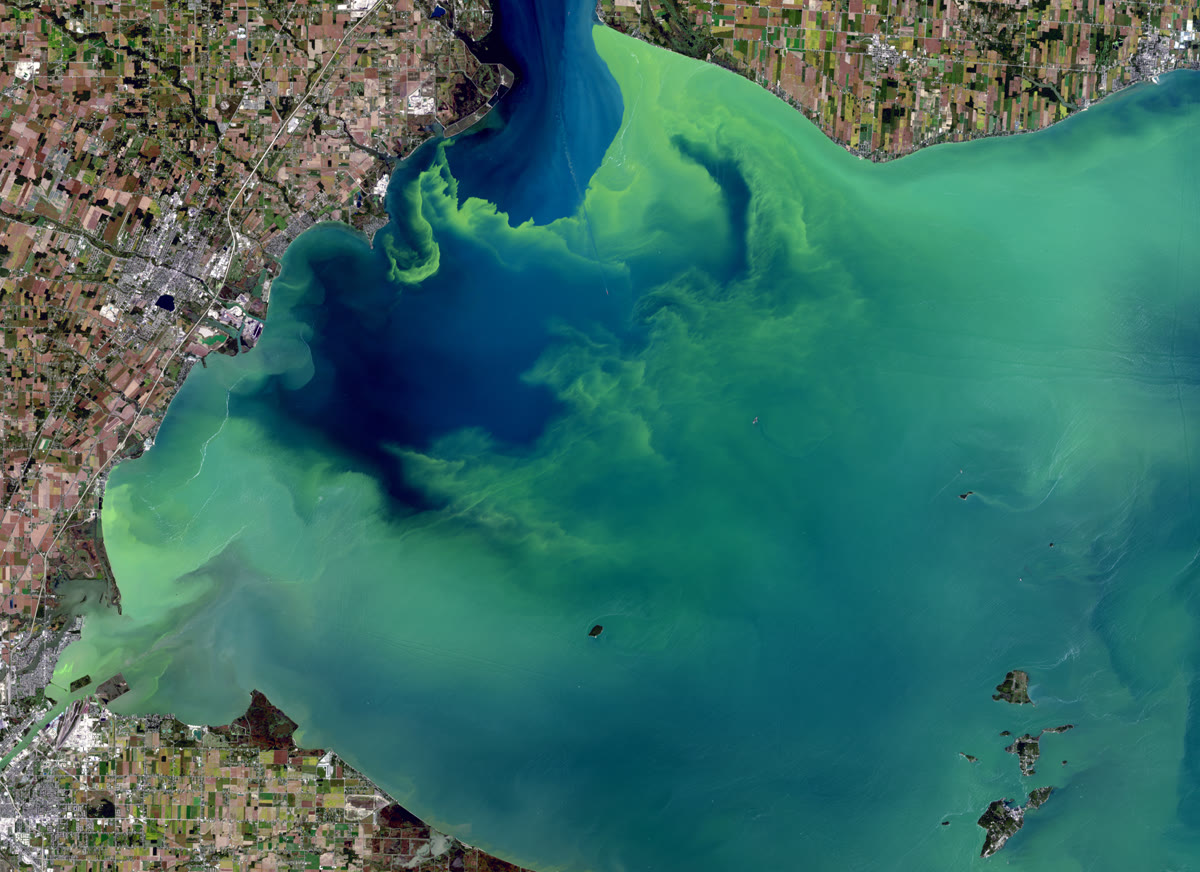
\includegraphics[width=0.62\linewidth]{images/book4/algal-bloom.jpg}

{\small Algenbloei op een groot meer, eind september gezien door een
aardobservatiesatelliet: de groene wervelingen zijn dichte populaties
microscopische algen, gevoed door voedingsstoffen uit de omliggende
landbouwgrond. Beeld: USGS en NASA, publiek domein.}
\end{omfigure}

\section{De atmosfeer}

\begin{definition}[Broeikasgassen]\label{def:b3:environmental-toxicology:greenhouse}
Een \emph{broeikasgas}\index{broeikasgas} absorbeert en zendt infrarode
straling uit bij de golflengten van de straling die het aardoppervlak
uitzendt, en warmt zo de lagere atmosfeer op. Het
\emph{aardopwarmingsvermogen}\index{aardopwarmingsvermogen} (GWP) van
een gas over een tijdshorizon, meestal 100 jaar, is de energie die het
vasthoudt na de uitstoot van één kilogram, ten opzichte van één kilogram
koolstofdioxide.
\end{definition}

Een molecuul absorbeert infrarode straling alleen via vibraties die zijn
dipoolmoment veranderen (\cref{ch:b3:group-theory-applied}). Distikstof
en dizuurstof, homonucleaire diatomische moleculen, hebben zo'n vibratie
niet en zijn doorzichtig; argon heeft helemaal geen vibratie.
Koolstofdioxide, lineair en apolair, heeft een IR-actieve buigvibratie
rond \qty{15}{\micro\metre}, midden in de emissie van de aarde; water,
methaan en distikstofoxide absorberen bij veel golflengten.

% ledger: atm:CO2.2025, atm:CH4.2025, atm:N2O.2025, gwp:CH4.fossil, gwp:CH4.nonfossil, gwp:N2O, life:CH4, life:N2O
In 2025 waren de wereldgemiddelde molfracties \qty{425.6}{ppm} koolstofdioxide, \qty{1936}{ppb}
methaan en \qty{338.9}{ppb} distikstofoxide. Methaan, dat door hydroxylradicalen
verwijderd wordt met een levensduur van ongeveer 12 jaar, heeft een
GWP-100 van 27 tot 30; distikstofoxide, dat alleen in de stratosfeer
afgebroken wordt met een levensduur van ongeveer 109 jaar, een GWP-100
van 273. Koolstofdioxide heeft geen
enkelvoudige levensduur: een deel van een uitstoot blijft eeuwenlang in
de lucht.

\begin{definition}[Luchtverontreinigende stoffen]\label{def:b3:environmental-toxicology:pollutants}
\emph{Fijnstof}\index{fijnstof} omvat de vaste en vloeibare deeltjes die
in de lucht zweven, ingedeeld naar aerodynamische diameter (fijne
deeltjes kleiner dan \qty{2.5}{\micro\metre} dringen diep in de longen
door). \emph{Zure regen}\index{zure regen} is regen die zuurder gemaakt
is dan schone regen door zwavelzuur en salpeterzuur, gevormd uit
zwaveldioxide en stikstofoxiden.
\end{definition}

\begin{proposition}[pH van schone regen]\label{prop:b3:environmental-toxicology:rain-ph}
Regen in evenwicht met het koolstofdioxide van de huidige lucht, en met
niets anders, heeft een pH van ongeveer 5.6.
\end{proposition}

\begin{proof}
% ledger: henry:CO2, pka4:H2CO3.1, pkw4:25C, const:atm
De wet van Henry geeft $[\ce{CO2(aq)}] = K_Hp(\ce{CO2}) = \qty{3.4e-7}{mol.L^{-1}.Pa^{-1}} \times (425.6 \times 10^{-6} \times \qty{101325}{Pa}) = \qty{1.47e-5}{mol/L}$. De
ladingsbalans is $[\ce{H+}] = [\ce{HCO3-}] + 2[\ce{CO3^2-}] + [\ce{OH-}] \approx K_{a1}[\ce{CO2(aq)}]/[\ce{H+}] + K_w/[\ce{H+}]$, dus
$[\ce{H+}]^2 = K_{a1}[\ce{CO2(aq)}] + K_w = 10^{-6.35} \times \num{1.47e-5} + 10^{-14} = \num{6.6e-12}$: $[\ce{H+}] = \qty{2.6e-6}{mol/L}$, pH 5.6.
\end{proof}

Zwaveldioxide uit de verbranding van zwavelhoudende brandstof en
stikstofoxiden uit hete verbranding worden in de lucht, door
hydroxylradicalen en in wolkendruppels, geoxideerd tot zwavelzuur en
salpeterzuur, die de regen tot pH 4 en lager brengen. Het verwijderen van
zwavel uit brandstoffen en van stikstofoxiden uit uitlaatgassen
(katalysatoren, ammoniakinjectie in elektriciteitscentrales) heeft het
probleem grotendeels opgelost waar het toegepast werd. Ozon aan de grond,
gevormd wanneer zonlicht inwerkt op stikstofoxiden en vluchtige
organische stoffen (\cref{ch:b3:photochemistry}), en fijne deeltjes
blijven de belangrijkste luchtverontreinigende stoffen voor de
gezondheid.

\section{Natuurlijke wateren}

\begin{omfigure}
\begin{tikzpicture}
\begin{axis}[name=a, width=0.48\linewidth, height=5.4cm, xmin=4, xmax=13, ymin=0, ymax=1.02,
  axis lines=left, xlabel={pH}, ylabel={fractie opgeloste koolstof},
  tick label style={font=\scriptsize}, label style={font=\small}]
\addplot[color=omDef, thick] table[x=pH, y=a0] {figdata/out/bachelor-3-carbonate-system.dat};
\addplot[color=omMeth, thick] table[x=pH, y=a1] {figdata/out/bachelor-3-carbonate-system.dat};
\addplot[color=omThm, thick] table[x=pH, y=a2] {figdata/out/bachelor-3-carbonate-system.dat};
\node[font=\scriptsize, omDef] at (axis cs:4.9,0.85) {$\ce{CO2(aq)}$};
\node[font=\scriptsize, omMeth] at (axis cs:8.3,0.88) {$\ce{HCO3-}$};
\node[font=\scriptsize, omThm] at (axis cs:12.1,0.85) {$\ce{CO3^2-}$};
\draw[black!30, dashed] (axis cs:6.35,0) -- (axis cs:6.35,0.5) (axis cs:10.33,0) -- (axis cs:10.33,0.5);
\end{axis}
\begin{axis}[at={(a.east)}, anchor=west, xshift=1.4cm, width=0.48\linewidth, height=5.4cm,
  xmin=0, xmax=2000, ymin=5.2, ymax=6.2, axis lines=left,
  xlabel={$\ce{CO2}$ in lucht / ppm}, ylabel={pH van de regen},
  tick label style={font=\scriptsize}, label style={font=\small},
  scaled x ticks=false, xticklabel style={/pgf/number format/1000 sep={}}]
\addplot[color=omDef, thick] table[x=ppm, y=pH] {figdata/out/bachelor-3-carbonate-system-b.dat};
\draw[black!35, dashed] (axis cs:425.6,5.2) -- (axis cs:425.6,5.59);
\node[font=\scriptsize, anchor=west] at (axis cs:470,5.63) {nu: 5.6};
\end{axis}
\end{tikzpicture}

{\small Links: verdeling van de opgeloste anorganische koolstof over zijn
drie vormen tegen de pH bij \qty{25}{\celsius}, met snijpunten bij $\mathrm pK_{a1} = 6.35$ en $\mathrm pK_{a2} = 10.33$. Rechts: pH van regen in
evenwicht met alleen koolstofdioxide, tegen zijn molfractie in de lucht.}
\end{omfigure}

\begin{proposition}[Carbonaatfracties]\label{prop:b3:environmental-toxicology:carbonate-fractions}
Met $C_T$ de totale opgeloste anorganische koolstof is
$[\ce{CO2(aq)}] = C_Th^2/D$, $[\ce{HCO3-}] = C_TK_{a1}h/D$, $[\ce{CO3^2-}] = C_TK_{a1}K_{a2}/D$, waarin $h = [\ce{H+}]$ en $D = h^2 + K_{a1}h + K_{a1}K_{a2}$.
\end{proposition}

\begin{proof}
Uit de twee zuurconstanten volgt
\[
  [\ce{HCO3-}] = \frac{K_{a1}[\ce{CO2(aq)}]}{h}, \qquad [\ce{CO3^2-}] = \frac{K_{a2}[\ce{HCO3-}]}{h} = \frac{K_{a1}K_{a2}[\ce{CO2(aq)}]}{h^2}.
\]
Hun som is $C_T = [\ce{CO2(aq)}]\,D/h^2$; elke vorm delen door $C_T$ geeft de fracties.
\end{proof}

\begin{definition}[Alkaliniteit]\label{def:b3:environmental-toxicology:alkalinity}
De \emph{alkaliniteit}\index{alkaliniteit} van een water is zijn vermogen
om sterk zuur te neutraliseren, gemeten door titratie tot het
equivalentiepunt van koolzuur (ongeveer pH
4.5) en uitgedrukt in mol $\ce{H+}$ per liter.
\end{definition}

\begin{proposition}[Carbonaatalkaliniteit]\label{prop:b3:environmental-toxicology:alkalinity}
In een water waarvan de basen carbonaatspecies en hydroxide zijn, is
$\mathrm{Alk} = [\ce{HCO3-}] + 2[\ce{CO3^2-}] + [\ce{OH-}] - [\ce{H+}]$; ze is gelijk aan het overschot van de ladingen van de kationen
van sterke basen over die van de anionen van sterke zuren, en verandert
niet wanneer koolstofdioxide met de lucht uitgewisseld wordt.
\end{proposition}

\begin{proof}
Titratie tot het equivalentiepunt van koolzuur zet elk $\ce{HCO3-}$ om in $\ce{CO2}$ (telkens één $\ce{H+}$),
elk $\ce{CO3^2-}$ in $\ce{CO2}$ (twee), elk $\ce{OH-}$ in water (één), terwijl het vrije $\ce{H+}$ dat al aanwezig is
negatief meetelt: de opgegeven som. De ladingsbalans van het water, met
$\ce{Na+}$, $\ce{Ca^2+}$\dots{} en $\ce{Cl-}$, $\ce{SO4^2-}$\dots, herschikt zich tot dezelfde som, gelijk aan $\sum z_i c_i$(kationen) $-$ $\sum z_jc_j$(anionen)
van de sterke elektrolyten. Het toevoegen of verwijderen van $\ce{CO2}$ verandert geen
van deze ionen.
\end{proof}

\begin{definition}[Verzuring van de oceaan]\label{def:b3:environmental-toxicology:acidification}
\emph{Verzuring van de oceaan}\index{verzuring van de oceaan} is de daling
van de pH van zeewater naarmate het koolstofdioxide uit de lucht opneemt.
De \emph{verzadigingstoestand}\index{verzadigingstoestand} van een
carbonaatmineraal is
$\Omega = [\ce{Ca^2+}][\ce{CO3^2-}]/K_{sp}$: boven 1 kan het mineraal ontstaan, onder 1 heeft het de neiging op te lossen.
\end{definition}

Opgelost koolstofdioxide zet carbonaationen om in waterstofcarbonaat, $\ce{CO2 + CO3^2- + H2O -> 2HCO3-}$,
wat de pH en $\Omega$ verlaagt: schelpen en koraalskeletten worden moeilijker te bouwen. (In
zeewater zijn de constanten schijnbare constanten, gemeten in het
zoutmilieu, die verschillen van de zoetwaterwaarden van dit hoofdstuk.)

\begin{definition}[Waterhardheid]\label{def:b3:environmental-toxicology:hardness}
De \emph{hardheid}\index{waterhardheid} van een water is zijn totale
concentratie calcium- en magnesiumionen, vaak uitgedrukt als de massa
calciumcarbonaat die hetzelfde aantal mol zou bevatten, in mg/L.
\end{definition}

\begin{definition}[Zuurstofverbruik]\label{def:b3:environmental-toxicology:oxygen-demand}
Het \emph{biochemisch zuurstofverbruik}\index{biochemisch zuurstofverbruik} (BZV) van een
water is de massa dizuurstof die per liter verbruikt wordt door
micro-organismen die zijn organische stof in het donker oxideren, over
een opgegeven tijd (vijf dagen bij \qty{20}{\celsius} voor $\mathrm{BZV_5}$). Zijn
\emph{chemisch zuurstofverbruik}\index{chemisch zuurstofverbruik} (CZV)
is de massa dizuurstof die equivalent is met het dichromaat dat verbruikt
wordt bij de chemische oxidatie van zijn organische stof.
\end{definition}

\begin{proposition}[BZV-kromme]\label{prop:b3:environmental-toxicology:bod}
Als biologisch afbreekbare organische stof volgens een kinetiek van de
eerste orde met snelheidsconstante $k$ verbruikt wordt, is de zuurstof die na de tijd $t$ verbruikt is $\mathrm{BZV}_t = L_0(1 - \eu^{-kt})$, waarin $L_0$ het uiteindelijke BZV is.
\end{proposition}

\begin{proof}
Het resterende verbruik $L$ voldoet aan $\dd L/\dd t = -kL$, dus $L = L_0\eu^{-kt}$; de verbruikte zuurstof is wat verdwenen is,
$L_0 - L$.
\end{proof}

\begin{omfigure}
\begin{tikzpicture}
\begin{axis}[name=a, width=0.48\linewidth, height=5.2cm, xmin=0, xmax=30, ymin=0, ymax=270,
  axis lines=left, xlabel={tijd / dagen}, ylabel={BZV / \unit{mg.L^{-1}}},
  tick label style={font=\scriptsize}, label style={font=\small}]
\addplot[color=omDef, thick] table[x=t, y=bod] {figdata/out/bachelor-3-bod.dat};
\draw[black!35, dashed] (axis cs:0,250) -- (axis cs:30,250);
\draw[black!35, dashed] (axis cs:5,0) -- (axis cs:5,170.8);
\node[font=\scriptsize, anchor=west] at (axis cs:5.6,140) {$\mathrm{BZV_5}$};
\node[font=\scriptsize, anchor=north east] at (axis cs:30,246) {$L_0$};
\end{axis}
\begin{axis}[at={(a.east)}, anchor=west, xshift=1.4cm, width=0.48\linewidth, height=5.2cm,
  xmin=0, xmax=15, ymin=0, ymax=10, axis lines=left,
  xlabel={tijd stroomafwaarts / dagen}, ylabel={opgelost $\ce{O2}$ / \unit{mg.L^{-1}}},
  tick label style={font=\scriptsize}, label style={font=\small}]
\addplot[color=omThm, thick] table[x=t, y=O2] {figdata/out/bachelor-3-bod-b.dat};
\draw[black!35, dashed] (axis cs:0,9.1) -- (axis cs:15,9.1);
\node[font=\scriptsize, anchor=south east] at (axis cs:15,9.1) {verzadiging};
\node[font=\scriptsize, anchor=north] at (axis cs:2.4,6.3) {kritiek punt};
\end{axis}
\end{tikzpicture}

{\small Links: het BZV van een modelafvalwater, $L_0 = \qty{250}{mg/L}$ en $k = \qty{0.23}{d^{-1}}$: ongeveer twee derde van het
verbruik gebeurt in vijf dagen. Rechts: de zuurstofdip in een rivier
onder een lozingspunt (model van Streeter-Phelps): de afbraak van de
organische belasting verbruikt in het begin zuurstof sneller dan de
lucht ze aanvult, tot het tekort na ongeveer 2.4 dagen een maximum
bereikt.}
\end{omfigure}

\begin{method}[Het CZV bepalen]\label{met:b3:environmental-toxicology:cod}
\begin{enumerate}
  \item Verhit een afgemeten volume monster onder reflux met een bekende
        overmaat kaliumdichromaat in zwavelzuur, met zilversulfaat als
        katalysator en kwik(II)sulfaat om chloride te binden.
  \item Titreer het resterende dichromaat met ijzer(II) met ferroïne, en
        voer een blanco uit met zuiver water.
  \item Het verbruikte dichromaat, omgerekend naar de equivalente massa $\ce{O2}$ (één
        $\ce{Cr2O7^2-}$ neemt zes elektronen op, zoals 1.5 $\ce{O2}$ zou doen), gedeeld door het volume van het monster, is het
        CZV in mg/L.
\end{enumerate}
\end{method}

\begin{definition}[Eutrofiëring]\label{def:b3:environmental-toxicology:eutrophication}
\emph{Eutrofiëring}\index{eutrofiering@eutrofiëring} is de verrijking van
een waterlichaam met voedingsstoffen, vooral fosfor en stikstof, die leidt
tot een overmatige groei van algen en planten, en daarna tot
zuurstofuitputting wanneer die afbreken.
\end{definition}

\begin{omfigure}
\begin{tikzpicture}[font=\scriptsize, >=Stealth,
  box/.style={draw, rounded corners, align=center, fill=omMeth!10, inner sep=3pt, minimum height=8mm}]
  \node[box] (f) at (-3.4,1.2) {akkers: kunstmest,\\ mest};
  \node[box] (t) at (-3.4,-0.4) {steden: afvalwater,\\ wasmiddelen};
  \node[box] (a) at (0,2.1) {atmosfeer:\\ depositie (N)};
  \node[box, fill=omDef!12, minimum width=3.2cm, minimum height=1.7cm] (l) at (0.6,0.4) {meerwater:\\ algen groeien};
  \node[box, fill=black!8] (s) at (0.6,-1.6) {sediment: P opgeslagen,\\ vrijgezet bij zuurstofloosheid};
  \node[box] (o) at (4.0,0.4) {afvoer};
  \draw[->, thick] (f) -- node[above, sloped, pos=0.4] {afspoeling} (l);
  \draw[->, thick] (t) -- node[below, sloped] {N, P} (l);
  \draw[->, thick] (a) -- (l);
  \draw[->, thick] (l) -- node[left] {dode algen} (s);
  \draw[->, thick, dashed] (s.east) to[bend right=30] node[right] {P} (l.south east);
  \draw[->, thick] (l) -- (o);
\end{tikzpicture}

{\small Stromen van voedingsstoffen naar en binnen een meer. Fosfor, in
zoet water vaak de beperkende voedingsstof, hoopt zich op in het sediment
en keert terug naar het water wanneer de bodem zijn zuurstof verliest,
wat de algenbloei jarenlang kan onderhouden nadat de aanvoer gestopt is.}
\end{omfigure}

Algen nemen koolstof, stikstof en fosfor op in ruwweg constante
verhoudingen; de voedingsstof die ten opzichte van die behoeften tekort
schiet, beperkt hun groei. In de meeste meren is dat fosfor, en daarom
werden fosfaten uit wasmiddelen en uit gezuiverd afvalwater verwijderd;
in veel kustzeeën is het stikstof.

\begin{definition}[Speciatie]\label{def:b3:environmental-toxicology:speciation}
De \emph{chemische speciatie}\index{chemische speciatie} van een element
in een monster is de verdeling van zijn hoeveelheid over zijn chemische
vormen: oxidatietoestanden, complexen, organometaalverbindingen, vrije en
gebonden species.
\end{definition}

De toxiciteit hangt af van de speciatie. Anorganisch kwik dat in water
terechtkomt, wordt door bacteriën in sedimenten gemethyleerd tot
methylkwik, dat membranen passeert, de zwavel van eiwitten bindt en zich
langs voedselketens concentreert; arseen is veel giftiger als arseniet,
As(III), dan als arsenaat, As(V), en veel minder giftig in de organische
vormen die in zeevruchten voorkomen. Een totale concentratie alleen zegt
weinig.

\begin{method}[Speciatie van een metaal in een water]\label{met:b3:environmental-toxicology:speciation}
\begin{enumerate}
  \item Som de aanwezige liganden op (hydroxide, carbonaat, chloride,
        sulfaat, organische stof) met hun concentraties en de pH.
  \item Schrijf de complexvormingsconstanten en de massabalans van het
        metaal op, zoals in het deel van jaar~1.
  \item Los op naar het vrije metaalion, daarna elk complex; teken de
        fracties tegen de pH of tegen een ligandconcentratie.
  \item Vergelijk de giftige of biologisch beschikbare vorm (vaak het
        vrije ion) met het totaal.
\end{enumerate}
\end{method}

\section{Bodems en sedimenten}

\begin{definition}[Sorptie in bodems]\label{def:b3:environmental-toxicology:soil}
De \emph{kationuitwisselingscapaciteit}\index{kationuitwisselingscapaciteit}
van een bodem is de hoeveelheid uitwisselbare kationen die hij per
massa-eenheid kan vasthouden, op kleien en organische stof. De
\emph{bodem-waterverdelingscoëfficiënt}\index{bodem-waterverdelingscoefficient@bodem-waterverdelingscoëfficiënt}
$K_d$ is de verhouding van de concentratie van een stof die op de bodem
gesorbeerd is (per kilogram) tot haar concentratie in het poriewater (per
liter); de
\emph{verdelingscoëfficiënt voor organische koolstof}\index{verdelingscoefficient voor organische koolstof@verdelingscoëfficiënt voor organische koolstof}
is $K_{oc} = K_d/f_{oc}$, met $f_{oc}$ de massafractie organische koolstof.
\end{definition}

Neutrale organische verbindingen sorberen vooral op de organische stof
van de bodem, zodat $K_{oc}$ veel minder van bodem tot bodem varieert dan $K_d$. Een verbinding met een kleine $K_d$ beweegt met het water
mee en kan het grondwater bereiken (uitloging); een verbinding met een grote $K_d$ blijft dicht bij het oppervlak,
gebonden aan deeltjes die erosie naar rivieren en meren kan voeren.

\section{Lot van verontreinigende stoffen}

\begin{definition}[Octanol-waterverdelingscoëfficiënt]\label{def:b3:environmental-toxicology:kow}
De \emph{octanol-waterverdelingscoëfficiënt}\index{octanol-waterverdelingscoefficient@octanol-waterverdelingscoëfficiënt}
$K_{ow}$ van een stof is de verhouding van haar evenwichtsconcentraties in
octaan-1-ol en in water; hij meet haar affiniteit voor vetweefsel en
organische stof.
\end{definition}

% ledger: logkow:DDT, logkow:benzene, logkow:atrazine, logkow:PCB153
Benzeen heeft $\log K_{ow} = 2.13$, het herbicide atrazine 2.61, een hexagechloreerd PCB 6.67 en
DDT 6.91: de laatste twee lossen tientallen miljoenen keren beter op in
vet dan in water.

\begin{definition}[Bioaccumulatie]\label{def:b3:environmental-toxicology:bio}
De \emph{bioconcentratiefactor}\index{bioconcentratiefactor} (BCF) is de
verhouding van de concentratie in een organisme tot die in het omringende
water in stationaire toestand, bij opname uit het water alleen.
\emph{Bioaccumulatie}\index{bioaccumulatie} is de ophoping in een
organisme langs alle wegen, voedsel inbegrepen;
\emph{biomagnificatie}\index{biomagnificatie} is de toename van de
concentratie van prooi naar roofdier langs een voedselketen.
\end{definition}

\begin{proposition}[BCF en $K_{ow}$]\label{prop:b3:environmental-toxicology:bcf-kow}
Voor neutrale organische stoffen die niet gemetaboliseerd worden, is $\log\mathrm{BCF}$ in vissen
bij benadering een lineaire functie van $\log K_{ow}$, met een helling dicht bij 1, tot $\log K_{ow}$ rond 6;
daarboven vertraagt de opname en vlakt het verband af (empirische
regressies).
\admitted
\end{proposition}

\begin{definition}[Persistente organische verontreinigende stoffen]\label{def:b3:environmental-toxicology:pop}
Een \emph{persistente organische verontreinigende stof}\index{persistente organische verontreinigende stof}
is een organische stof die afbraak weerstaat, bioaccumuleert, giftig is
en ver van haar bronnen vervoerd wordt, zoals DDT, de PCB's en de
dioxinen.
\end{definition}

\begin{proposition}[Evenwichtsverdeling over compartimenten]\label{prop:b3:environmental-toxicology:level-one}
Een massa $M$ van een stof die in evenwicht verdeeld is (een model van ``niveau I'') over water
(volume $V_w$), lucht ($V_a$), vaste sedimentdeeltjes ($m_s$) en vis ($m_f$) heeft de waterconcentratie
$C_w = M/(V_w + K_{aw}V_a + K_{sw}m_s + K_{fw}m_f)$, waarin de $K$ de verdelingscoëfficiënten ten opzichte van
water zijn; de massa in elk compartiment is zijn term maal $C_w$.
\end{proposition}

\begin{proof}
In evenwicht is $C_a = K_{aw}C_w$, $C_s = K_{sw}C_w$ (per kilogram), $C_f = K_{fw}C_w$. De massabalans is
$M = C_wV_w + C_aV_a + C_sm_s + C_fm_f = C_w(V_w + K_{aw}V_a + K_{sw}m_s + K_{fw}m_f)$; delen geeft $C_w$.
\end{proof}

\begin{omfigure}
\begin{tikzpicture}[font=\scriptsize, >=Stealth,
  comp/.style={draw, rounded corners, align=center, minimum width=2.6cm, minimum height=1.0cm}]
  \node[comp, fill=omDef!8] (air) at (0,2.2) {lucht\\ $C_a = K_{aw}C_w$};
  \node[comp, fill=omDef!25] (w) at (0,0.6) {water\\ $C_w$};
  \node[comp, fill=black!10] (sed) at (0,-1.0) {sediment\\ $C_s = K_{sw}C_w$};
  \node[comp, fill=omMeth!15] (fish) at (3.6,0.6) {vis\\ $C_f = K_{fw}C_w$};
  \node[comp, fill=omProp!15] (soil) at (-3.6,0.6) {bodem\\ $C_{soil} = K_dC_w$};
  \draw[<->, thick] (air) -- (w); \draw[<->, thick] (w) -- (sed);
  \draw[<->, thick] (w) -- (fish); \draw[<->, thick] (w) -- (soil);
\end{tikzpicture}

{\small Compartimenten van een evenwichtsmodel (niveau I): elk
compartiment is in evenwicht met het water, en zijn concentratie ligt
vast door een verdelingscoëfficiënt. De stof hoopt zich op waar het
product van capaciteit en volume (of massa) het grootst is, voor een
hydrofobe verbinding vaak het sediment of de bodem.}
\end{omfigure}

\section{Toxicologie en regelgeving}

\begin{definition}[Dosis-respons]\label{def:b3:environmental-toxicology:dose}
Een \emph{dosis-responsrelatie}\index{dosis-responsrelatie} verbindt de
dosis van een stof met de grootte of de frequentie van een effect. De
\emph{mediane letale dosis}\index{mediane letale dosis} $\mathrm{LD_{50}}$ doodt de helft van een testpopulatie; de
\emph{mediane effectieve concentratie}\index{mediane effectieve concentratie} $\mathrm{EC_{50}}$
veroorzaakt een opgegeven effect bij de helft. Het
\emph{niveau zonder waargenomen schadelijk
effect}\index{niveau zonder waargenomen schadelijk effect} (NOAEL) is de
hoogste geteste dosis zonder schadelijk effect, het
\emph{laagste niveau met waargenomen schadelijk
effect}\index{laagste niveau met waargenomen schadelijk effect} (LOAEL) de
laagste geteste dosis met zo'n effect.
\end{definition}

\begin{proposition}[Log-logistisch model]\label{prop:b3:environmental-toxicology:dose-response}
In het log-logistische model $f(d) = 1/\bigl(1 + (D_{50}/d)^n\bigr)$ is de respons de helft bij $d = D_{50}$, en meet $n$
de steilheid: de verhouding van de doses voor 10\,\% en 90\,\% respons is $81^{1/n}$.
\end{proposition}

\begin{proof}
Bij $d = D_{50}$ is $f = 1/2$. $f = 0.1$ vereist $(D_{50}/d)^n = 9$, $f = 0.9$ vereist $(D_{50}/d)^n = 1/9$; de verhouding van de twee doses
is $(9 \times 9)^{1/n} = 81^{1/n}$.
\end{proof}

\begin{omfigure}
\begin{tikzpicture}
\begin{axis}[width=0.72\linewidth, height=5.4cm, xmode=log, xmin=3, xmax=3200, ymin=0, ymax=1.02,
  axis lines=left, xlabel={dosis / \unit{mg.kg^{-1}}}, ylabel={fractie met respons},
  tick label style={font=\scriptsize}, label style={font=\small}]
\addplot[color=omDef, thick] table[x=d, y=n2] {figdata/out/bachelor-3-dose-response.dat};
\addplot[color=omThm, thick] table[x=d, y=n6] {figdata/out/bachelor-3-dose-response.dat};
\addplot[only marks, mark=*, mark size=1.6pt, omThm] table[x=d, y=r] {figdata/out/bachelor-3-dose-response-b.dat};
\draw[black!35, dashed] (axis cs:200,0) -- (axis cs:200,0.5) -- (axis cs:3,0.5);
\node[font=\scriptsize, anchor=north west] at (axis cs:200,0.48) {$D_{50}$};
\node[font=\scriptsize, omThm, anchor=south east, inner sep=1pt] (noael) at (axis cs:60,0.09) {NOAEL};
\draw[omThm] (noael.south east) -- (axis cs:78,0.012);
\node[font=\scriptsize, omThm, anchor=west] at (axis cs:165,0.2) {LOAEL};
\node[font=\scriptsize, omDef, anchor=east] at (axis cs:60,0.25) {$n = 2$};
\node[font=\scriptsize, omThm, anchor=east] at (axis cs:185,0.8) {$n = 6$};
\end{axis}
\end{tikzpicture}

{\small Log-logistische dosis-responskrommen met dezelfde mediane dosis
(\qty{200}{mg/kg}, model) en twee steilheden. De stippen zijn een studie
bij vijf doses voor de steilere kromme: met een respons van 5\,\% als
criterium voor een schadelijk effect is de NOAEL
\qty{80}{mg/kg} en de LOAEL \qty{160}{mg/kg}; beide hangen af van de gekozen doses.}
\end{omfigure}

\begin{definition}[Acute en chronische toxiciteit]\label{def:b3:environmental-toxicology:toxicity}
\emph{Acute toxiciteit}\index{acute toxiciteit} is de schade die een
enkele blootstelling of blootstellingen binnen een korte tijd
veroorzaken; \emph{chronische toxiciteit}\index{chronische toxiciteit} de
schade door herhaalde of voortdurende blootstelling gedurende een groot
deel van een leven.
\end{definition}

% ledger: ld50:NaCl, ld50:caffeine, ld50:nicotine
Toxiciteit is een kwestie van dosis: de orale $\mathrm{LD_{50}}$ bij ratten is ongeveer \qty{3000}{mg/kg} voor natriumchloride,
\qty{192}{mg/kg} voor cafeïne en \qty{188}{mg/kg} voor nicotine in hetzelfde soort gegevens. Voor de
meeste effecten bestaat er een drempeldosis waaronder het lichaam zich
redt; voor genotoxische kankerverwekkende stoffen wordt er geen
aangenomen, en wordt de blootstelling zo laag gehouden als redelijkerwijs
haalbaar is.

\begin{definition}[Ecotoxicologie]\label{def:b3:environmental-toxicology:ecotoxicology}
\emph{Ecotoxicologie}\index{ecotoxicologie} bestudeert de effecten van
stoffen op organismen in ecosystemen. De
\emph{voorspelde concentratie zonder effect}\index{voorspelde concentratie zonder effect}
(PNEC) is de laagste concentratie met of zonder effect uit testen op
representatieve soorten, gedeeld door een beoordelingsfactor die de
onzekerheid dekt; de
\emph{voorspelde milieuconcentratie}\index{voorspelde milieuconcentratie}
(PEC) is de concentratie die verwacht wordt uit het gebruik en het lot
van de stof; het \emph{risicoquotiënt}\index{risicoquotient@risicoquotiënt}
is PEC/PNEC.
\end{definition}

\begin{proposition}[Risicoquotiënt]\label{prop:b3:environmental-toxicology:risk-quotient}
Een \omterm{def:b3:environmental-toxicology:ecotoxicology}{risicoquotiënt} onder 1 wijst op geen zorg voor het beoordeelde
compartiment; boven 1 op een risico dat verfijnde gegevens of maatregelen
om de blootstelling te verminderen vereist.
\end{proposition}

\begin{proof}[Per definitie]
De PNEC wordt via haar beoordelingsfactor onder de concentraties gelegd
waarbij effecten waargenomen werden; een verwachte concentratie eronder
zal dus naar verwachting geen effecten veroorzaken, en een concentratie
erboven wel.
\end{proof}

\begin{method}[Een milieurisicobeoordeling]\label{met:b3:environmental-toxicology:risk}
\begin{enumerate}
  \item Gevaar: verzamel toxiciteitsgegevens voor algen, ongewervelden en
        vissen (acute
        $\mathrm{EC_{50}}$, chronische NOEC); neem de laagste; deel door de beoordelingsfactor (groter als
        er alleen acute gegevens zijn) om de PNEC te krijgen.
  \item Blootstelling: bereken uit de gebruikte hoeveelheden en het lot
        (verdeling, afbraak) de PEC in elk compartiment, of meet ze.
  \item Risico: bereken PEC/PNEC; verfijn boven 1 de gegevens of verminder
        de blootstelling, en herhaal.
\end{enumerate}
\end{method}

\begin{definition}[Grenswaarde voor beroepsmatige blootstelling]\label{def:b3:environmental-toxicology:oel}
Een
\emph{grenswaarde voor beroepsmatige blootstelling}\index{grenswaarde voor beroepsmatige blootstelling}
is de concentratie van een stof in de lucht van een werkplek die
werknemers mogen inademen, gemiddeld over een werkdag (of over 15 minuten
voor kortetermijnwaarden), zonder verwachte schadelijke effecten.
\end{definition}

Nieuwe chemische stoffen die in grote hoeveelheden op een markt gebracht
worden, moeten geregistreerd worden met een dossier over hun
eigenschappen, gevaren en toepassingen; de gevaarlijkste kunnen beperkt
of alleen voor toegelaten toepassingen gebruikt worden.

\begin{inthelab}[$\mathrm{BZV_5}$ meten]
Een monster wordt verdund met belucht verdunningswater dat
voedingsstoffen en een bacterieel entmateriaal bevat, zodat een groot
deel, maar niet alles, van de zuurstof verbruikt zal worden. Twee
afgesloten flessen worden tot de rand gevuld: de opgeloste zuurstof van
de ene wordt meteen gemeten met een zuurstofelektrode, die van de andere
na vijf dagen in het donker bij
\qty{20}{\celsius}. Het verschil, maal de verdunningsfactor en
gecorrigeerd voor het entmateriaal, is het
$\mathrm{BZV_5}$.
\end{inthelab}

\begin{safety}{\ghs[0.62cm]{GHS03}\ghs[0.62cm]{GHS05}\ghs[0.62cm]{GHS06}\ghs[0.62cm]{GHS08}\ghs[0.62cm]{GHS09}}
% ledger: ghs:K2Cr2O7, ghs4:HgSO4
De reagentia voor het CZV: kaliumdichromaat is oxiderend, kan kanker en
genetische defecten veroorzaken, is bijtend en sensibiliserend;
kwik(II)sulfaat is dodelijk bij inslikken, inademing of contact met de
huid en zeer giftig voor in het water levende organismen. Beide worden
in afgesloten buisjes gebruikt, en de gebruikte buisjes gaan naar het
gevaarlijk afval.
\end{safety}

\begin{history}[Een boek en een baai]
In 1962 beschreef \textit{Silent Spring} van Rachel Carson de achteruitgang
van vogels die vergiftigd werden door DDT en andere pesticiden die zich
langs voedselketens concentreren, en gaf het de aanzet tot de moderne
milieuregelgeving. Enkele jaren eerder, in 1956, werd bij de bewoners van
de baai van Minamata een ziekte van het zenuwstelsel herkend: een
chemische fabriek had methylkwik geloosd, gevormd uit haar
kwikkatalysator, dat zich ophoopte in de vis die de inwoners aten.
\end{history}

\section{Oefeningen}

\begin{exercise}[$\star$]\label{exo:b3:environmental-toxicology:1}
Waarom absorberen $\ce{N2}$, $\ce{O2}$ en Ar niet in het infrarood, en welke vibratie van $\ce{CO2}$ maakt er een
\omterm{def:b3:environmental-toxicology:greenhouse}{broeikasgas} van?
\end{exercise}

\begin{exercise}[$\star$]\label{exo:b3:environmental-toxicology:2}
Met welke factor verandert $[\ce{H+}]$ wanneer de pH van zeewater met 0.1 daalt?
\end{exercise}

\begin{exercise}[$\star$]\label{exo:b3:environmental-toxicology:3}
Een water bevat \qty{2.0}{mmol/L} $\ce{Ca^2+}$ en \qty{0.50}{mmol/L} $\ce{Mg^2+}$. Geef zijn \omterm{def:b3:environmental-toxicology:hardness}{hardheid} in mg $\ce{CaCO3}$ per liter.
\end{exercise}

\begin{exercise}[$\star$]\label{exo:b3:environmental-toxicology:4}
Algen nemen C, N en P op in de molverhouding $106 : 16 : 1$ (gegevens van de oefening). Een meerwater
bevat \qty{0.60}{mg/L} nitraatstikstof en \qty{0.010}{mg/L} fosfaatfosfor. Welke voedingsstof beperkt
de groei?
\end{exercise}

\begin{exercise}[$\star\star$]\label{exo:b3:environmental-toxicology:5}
Een $\mathrm{BZV_5}$ van \qty{170}{mg/L} wordt gemeten op een afvalwater met $k = \qty{0.23}{d^{-1}}$. Schat zijn uiteindelijke BZV.
\end{exercise}

\begin{exercise}[$\star\star$]\label{exo:b3:environmental-toxicology:6}
Een watermonster van \qty{100.0}{mL} vereist \qty{4.40}{mL} zoutzuur van \qty{0.0200}{mol/L} om pH 4.5 te bereiken. Bereken zijn
\omterm{def:b3:environmental-toxicology:alkalinity}{alkaliniteit} en, als ze volledig uit waterstofcarbonaat bestaat, de
concentratie daarvan in mg/L.
\end{exercise}

\begin{exercise}[$\star\star$]\label{exo:b3:environmental-toxicology:7}
Een bodem heeft $f_{oc} = 0.020$; een pesticide heeft $K_{oc} = \qty{300}{L/kg}$ (gegevens van de oefening). Bereken $K_d$ en de
fractie van het pesticide die gesorbeerd is in een bodem met \qty{1.5}{kg} vaste stof per \qty{0.30}{L} poriewater.
\end{exercise}

\begin{exercise}[$\star\star$]\label{exo:b3:environmental-toxicology:8}
Schat met $\log\mathrm{BCF} = 0.85\log K_{ow} - 0.70$ (een empirische regressie, gegevens van de oefening) de BCF van
benzeen en van een hexagechloreerd PCB, en becommentarieer.
\end{exercise}

\begin{exercise}[$\star\star$]\label{exo:b3:environmental-toxicology:9}
Druk de orale $\mathrm{LD_{50}}$ van cafeïne bij ratten uit als massa voor een volwassene van \qty{70}{kg} en als koppen koffie van
\qty{90}{mg} elk (een naïeve omrekening, gegevens van de oefening). Waarom is zo'n omrekening
slechts indicatief?
\end{exercise}

\begin{exercise}[$\star\star\star$]\label{exo:b3:environmental-toxicology:10}
Een stof heeft een $\mathrm{EC_{50}}$ na 48 uur van \qty{0.50}{mg/L} voor watervlooien, een $\mathrm{EC_{50}}$ na 72 uur van \qty{1.2}{mg/L} voor algen
en een $\mathrm{LC_{50}}$ na 96 uur van \qty{2.0}{mg/L} voor vissen, allemaal acuut, en er geldt een beoordelingsfactor van 1000
(gegevens van de oefening). Bereken de PNEC, en het \omterm{def:b3:environmental-toxicology:ecotoxicology}{risicoquotiënt} voor een PEC van \qty{0.20}{\micro g/L}.
\end{exercise}

\begin{exercise}[$\star\star\star$]\label{exo:b3:environmental-toxicology:11}
Een visetende vogel eet vis met \qty{0.30}{mg/kg} van een persistente verontreinigende stof; de vissen eten
plankton met \qty{0.015}{mg/kg}; het water bevat \qty{2.0}{ng/L}. Bereken de bioconcentratie- en
biomagnificatiefactoren langs de keten als het vet van de vogel \qty{6.0}{mg/kg} bevat (gegevens van de
oefening).
\end{exercise}

\begin{exercise}[$\star\star\star$]\label{exo:b3:environmental-toxicology:12}
Een elektriciteitscentrale stoot \qty{1000}{t} $\ce{SO2}$ per jaar uit. Bereken de massa zwavelzuur die daaruit kan ontstaan,
en het volume regen dat het tot pH 4.0 zou brengen als alles met de
regen neerviel (verwaarloos andere zuren en basen).
\end{exercise}

\section{Probleem: een pesticide in een meer}

\begin{problem}[{Weekendprobleem --- een pesticide in een meer: zijn
verdeling over sediment en vis, een massabalans in evenwicht, zijn
afbraak over een jaar, en het risicoquotiënt voor de organismen van het
meer}]
\label{pb:b3:environmental-toxicology:1}
Gegevens van het probleem. Een meer bevat $\qty{1.0e9}{L}$ water onder $\qty{1.0e12}{L}$ lucht (de gemengde laag erboven),
met $\qty{1.0e8}{kg}$ vaste deeltjes van actief sediment ($f_{oc} = 0.040$) en $\qty{1.0e4}{kg}$ vis (lipidefractie 0.048).
Een pesticide heeft $\log K_{ow} = 4.0$, een lucht-waterverdelingscoëfficiënt $K_{aw} = \num{1.0e-4}$, en $K_{oc} = 0.41\,K_{ow}$;
$K_{fw}$ = lipidefractie $\times K_{ow}$. Er komt 100 kg van in het meer. Zijn halveringstijd in het meer is 60 dagen.
De gevoeligste chronische test geeft een NOEC van \qty{50}{\micro g/L}, met een beoordelingsfactor van 10;
vis voor menselijke consumptie mag niet meer dan \qty{1.0}{mg/kg} bevatten.

\medskip\noindent\textbf{Deel I --- Verdelingscoëfficiënten.}
\begin{enumerate}
  \item Wat zegt $\log K_{ow} = 4.0$ over het pesticide?
  \item Bereken $K_{oc}$ en de sediment-watercoëfficiënt $K_{sw}$.
  \item Bereken de vis-watercoëfficiënt $K_{fw}$.
  \item Is het pesticide vluchtig uit water? Gebruik $K_{aw}$.
  \item Waarom bepaalt organische koolstof, en niet minerale stof, zijn
        sorptie?
  \item Welk compartiment zal er naar verwachting het meest van bevatten?
\end{enumerate}

\medskip\noindent\textbf{Deel II --- Massabalans in evenwicht.}
\begin{enumerate}[resume]
  \item Bereken de capaciteitstermen $V_w$, $K_{aw}V_a$, $K_{sw}m_s$ en $K_{fw}m_f$.
  \item Bereken de waterconcentratie.
  \item Bereken de massa in elk compartiment.
  \item Bereken de concentraties in lucht, sediment en vis.
  \item Welke aanname van het model is het minst realistisch?
  \item Hoe zou afbraak het beeld veranderen (modellen van niveau II en
        III)?
\end{enumerate}

\medskip\noindent\textbf{Deel III --- Afbraak.}
\begin{enumerate}[resume]
  \item Bereken de snelheidsconstante van de eerste orde.
  \item Bereken de fractie die na één jaar overblijft.
  \item Bereken de waterconcentratie na één jaar.
  \item Waarom kan het sediment het pesticide langer vasthouden dan de
        halveringstijd doet vermoeden?
  \item Wat maakt een pesticide persistent?
\end{enumerate}

\medskip\noindent\textbf{Deel IV --- Risico.}
\begin{enumerate}[resume]
  \item Bereken de PNEC.
  \item Neem de begin-waterconcentratie als PEC: bereken het \omterm{def:b3:environmental-toxicology:ecotoxicology}{risicoquotiënt}.
  \item Trek een besluit voor de organismen van het meer.
  \item Vergelijk de concentratie in de vis met de consumptiedrempel.
  \item Wat zou je hierna meten, en waar?
  \item Welke maatregelen zouden de PEC verlagen?
  \item Waarom is de beoordelingsfactor zo belangrijk?
  \item Formuleer het resultaat: het \omterm{def:b3:environmental-toxicology:ecotoxicology}{risicoquotiënt} PEC/PNEC.
\end{enumerate}
\end{problem}
